\documentclass[a4paper,12pt]{article}
\usepackage{fontspec} % Пакет для работы со шрифтами в XeLaTeX
\setmainfont{Liberation Serif} % Теперь эта команда сработает
\usepackage[russian]{babel}
\usepackage{amsmath, amsfonts, amssymb}
\usepackage{geometry}
\usepackage{booktabs}
\usepackage{graphicx}
\usepackage{float}

\geometry{left=1cm,right=1cm,top=1cm,bottom=1cm}

\begin{document}

% --- ТИТУЛЬНЫЙ ЛИСТ ---
\begin{titlepage}
    \centering
    \textbf{Министерство науки и высшего образования Российской Федерации}\\
    ФЕДЕРАЛЬНОЕ ГОСУДАРСТВЕННОЕ АВТОНОМНОЕ ОБ ОБРАЗОВАТЕЛЬНОЕ\\
    УЧРЕЖДЕНИЕ ВЫСШЕГО ОБРАЗОВАНИЯ\\
    \textbf{НАЦИОНАЛЬНЫЙ ИССЛЕДОВАТЕЛЬСКИЙ УНИВЕРСИТЕТ ИТМО}\\
    \vspace{1cm}
    Факультет безопасности информационных технологий\\
    \vspace{2cm}
    Дисциплина:\\
    «Электротехника»\\
    \vspace{2cm}
    \textbf{ОТЧЕТ ПО ЛАБОРАТОРНОЙ РАБОТЕ №4}\\
    «Исследование переходных процессов в электрическоих цепях» \\
    \vspace{3cm}
    \begin{flushright}
        \textbf{Выполнил:}\\
        Пахомов Владимир Юрьевич, студент группы N3250\\
        \vspace{0.5cm}
        \textbf{Проверил:}\\
        Кононова Мария Евгеньевна\\
    \end{flushright}
    \vfill
    Санкт-Петербург\\
    2026
\end{titlepage}


\newpage


\textbf{Цель работы:} \\
Исследование переходных процессов в электрических цепях первого и второго порядков с источником постоянного напряжения, определение параметров схем замещения и сравнение экспериментальных данных с расчетными.

\textbf{Исходные данные (Вариант №22):}
\begin{itemize}
    \item Напряжение источника: $E = 11.500$ В
    \item Сопротивление резистора: $R = 230.000$ Ом
    \item Индуктивность: $L = 10.580$ Гн
    \item Емкость: $C = 200.000$ мкФ
\end{itemize}



\subsection*{Часть 1: Исследование переходных процессов в цепях первого порядка}

\subsubsection*{1.1 Исследование переходного процесса в RC-цепи}

\begin{figure}[H]
    \centering
    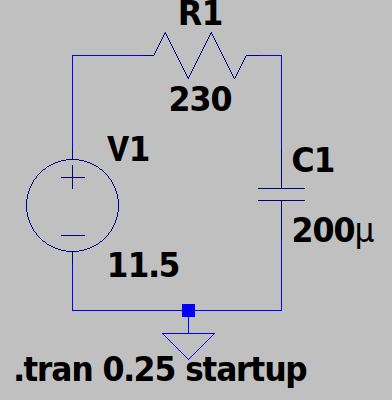
\includegraphics[width=9cm]{scheme1_1.png}
    \caption{Схема цепи}
\end{figure}

\textbf{Расчет теоретических значений:}
\begin{enumerate}
    \item Постоянная времени: $\tau_{calc} = R \cdot C = 230 \cdot 200 \cdot 10^{-6} = 0.046$ с = $46000$ мкс.
    \item Начальное значение тока: $I(0^+) = \frac{E}{R} = \frac{11.5}{230} = 0.050$ А = $50.000$ мА.
    \item Установившееся значение напряжения на конденсаторе: $U_C(\infty) = E = 11.500$ В.
\end{enumerate}

\textbf{Обработка экспериментальных данных:} \\
По результатам моделирования в LTspice:
\begin{itemize}
    \item Напряжение $U_C$ достигает $50\%$ от амплитуды ($5.750$ В) в момент времени $t_{0.5} \approx 31941.9$ мкс.
    \item Экспериментальная постоянная времени: $\tau_{exp} \approx 1.44 \cdot t_{0.5} = 1.44 \cdot 31941.9 \approx 45996.3$ мкс.
\end{itemize}

\begin{table}[H]
\centering
\caption{Результаты исследования RC-цепи (Таблица 4.2)}
\begin{tabular}{|c|c|c|c|c|c|c|c|}
\hline
$R$, [Ом] & $C$, [мкФ] & Тип данных & $I(0^+)$, [мА] & $I(\infty)$, [мА] & $U_C(0^+)$, [В] & $U_C(\infty)$, [В] & $\tau$, [мкс] \\
\hline

230.000 & 200.000 & эксп. & 49.989 & 0.218 & 0.002 & 11.450 & 45996.336 \\
\hline

 &  & расч. & 50.000 & 0.000 & 0.000 & 11.500 & 46000.000 \\ 
\hline

\end{tabular}
\end{table}


\begin{figure}[H]
    \centering
    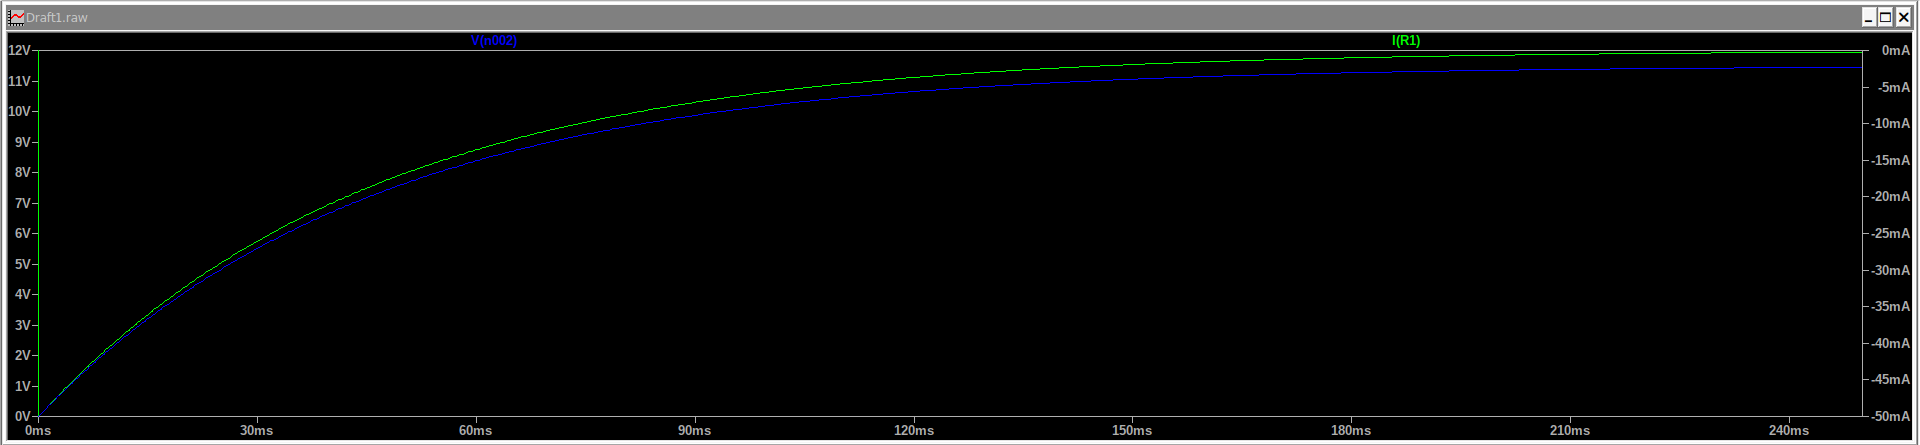
\includegraphics[width=19cm]{graphic1_1.png}
    \caption{График}
\end{figure}

\subsubsection*{1.2 Исследование переходного процесса в RL-цепи}


\textbf{Расчет теоретических значений:}
\begin{enumerate}
    \item Постоянная времени: $\tau_{calc} = \frac{L}{R} = \frac{10.58}{230} = 0.046$ с = $46000$ мкс.
    \item Начальное значение напряжения на катушке: $U_L(0^+) = E = 11.500$ В.
    \item Установившееся значение тока: $I(\infty) = \frac{E}{R} = \frac{11.5}{230} = 0.050$ А = $50.000$ мА.
\end{enumerate}

\textbf{Обработка экспериментальных данных:} \\
По результатам моделирования:
\begin{itemize}
    \item Напряжение на катушке $U_L$ спадает до $50\%$ ($5.750$ В) в момент времени $t_{0.5} \approx 31835.0$ мкс.
    \item Экспериментальная постоянная времени: $\tau_{exp} \approx 1.44 \cdot 31835.0 \approx 45842.4$ мкс.
\end{itemize}

\begin{table}[H]
\centering
\caption{Результаты исследования RL-цепи (Таблица 4.3)}
\begin{tabular}{|c|c|c|c|c|c|c|c|c|}
\hline
$R$, [Ом] & $L$, [мГн] & Тип данных & $I(0^+)$, [мА] & $I(\infty)$, [мА] & $U_L(0^+)$, [В] & $U_L(\infty)$, [В] & $\tau$, [мкс] \\
\hline
230 & 10580  & эксп. & 0.011 & 50.224 & 11.497 & 0.065 & 45842.400 \\
\hline
 &  & расч. & 0.000 & 50.000 & 11.500 & 0.000 & 46000.000  \\
\hline
\end{tabular}
\end{table}

\textbf{Пример расчета для RL-цепи:} \\
Согласно закону коммутации $i_L(0^-) = i_L(0^+) = 0$.
Тогда в момент $t=0^+$ по второму закону Кирхгофа:
$E = U_R + U_L \Rightarrow 11.5 = 0 \cdot 230 + U_L(0^+) \Rightarrow U_L(0^+) = 11.5$ В.
В установившемся режиме ($t \to \infty$) катушка представляет собой короткое замыкание (при $R_k=0$):
$I(\infty) = \frac{E}{R} = \frac{11.5}{230} = 0.05$ А.

\begin{figure}[H]
    \centering
    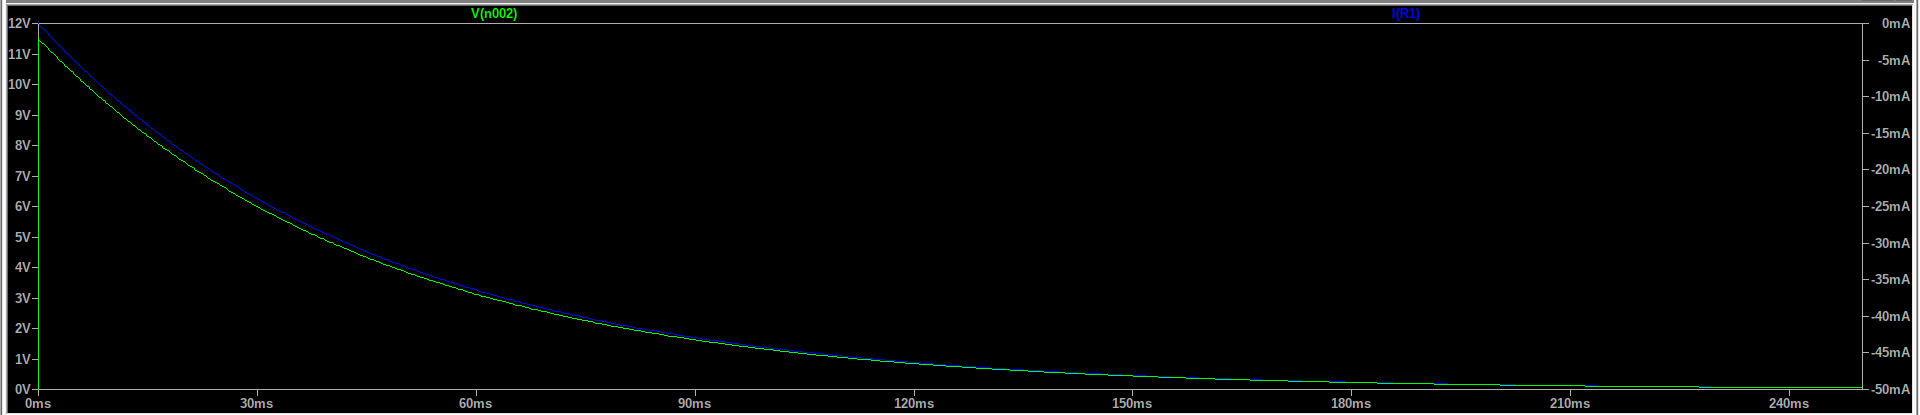
\includegraphics[width=19cm]{graphic1_2.png}
    \caption{График}
\end{figure}

\newpage


\subsection*{Часть 2: Исследование переходных процессов в цепи второго порядка}

В данной части исследуется последовательная RLC-цепь. Характер процесса зависит от соотношения между сопротивлением $R$ и критическим сопротивлением $R_{kp} = 2\sqrt{L/C}$.

\begin{figure}[H]
    \centering
    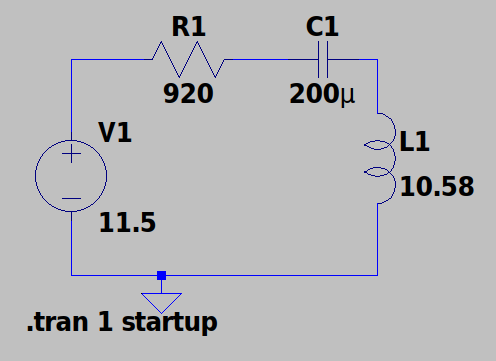
\includegraphics[width=12cm]{scheme2_1.png}
    \caption{Схема цепи}
\end{figure}

\subsubsection*{2.1 Расчет теоретических параметров}
\begin{enumerate}
    \item Характеристическое сопротивление: $\rho = \sqrt{\frac{10.58}{200 \cdot 10^{-6}}} = 230.000$ Ом.
    \item Резонансная частота: $\omega_0 = \frac{1}{\sqrt{LC}} = \frac{1}{\sqrt{10.58 \cdot 0.0002}} = 21.739$ рад/с.
    \item Коэффициент затухания для опыта 2.1 ($R=920$ Ом): $\delta = \frac{R}{2L} = \frac{920}{2 \cdot 10.58} = 43.478$ с$^{-1}$.
    \item Коэффициент затухания для опыта 2.2 ($R=115$ Ом): $\delta = \frac{115}{2 \cdot 10.58} = 5.435$ с$^{-1}$.
    \item Частота свободных колебаний (опыт 2.2): $\omega_c = \sqrt{\omega_0^2 - \delta^2} = \sqrt{21.739^2 - 5.435^2} = 21.049$ рад/с.
\end{enumerate}

\subsubsection*{2.2 Апериодический переходный процесс (Опыт 2.1, $R = 920$ Ом)}
В этом режиме $R > 2\rho$. Корни характеристического уравнения вещественные:
$s_{1,2} = -\delta \pm \sqrt{\delta^2 - \omega_0^2} = -43.478 \pm 37.653$.
$s_1 = -5.825$ с$^{-1}$, $s_2 = -81.131$ с$^{-1}$.
Время переходного процесса: $t_p \approx \frac{3}{|s_1|} = \frac{3}{5.825} = 0.515$ с = $515000$ мкс.

\subsubsection*{2.3 Колебательный переходный процесс (Опыт 2.2, $R = 115$ Ом)}
В этом режиме $R < 2\rho$. Из анализа файла \texttt{part3\_2\_2.txt}:
\begin{itemize}
    \item Первый пик тока $I_{m1} = 5.371$ мА при $t_1 = 0.034$ с.
    \item Второй однонаправленный пик $I_{m2} = 2.587$ мА при $t_2 = 0.334$ с.
    \item Период колебаний $T = t_2 - t_1 = 0.300$ с.
    \item Экспериментальное затухание: $\delta_{exp} = \frac{\ln(I_{m1}/I_{m2})}{T} = \frac{\ln(5.371/2.587)}{0.300} = 2.434$ с$^{-1}$.
    \item Экспериментальная частота: $\omega_{c,exp} = \frac{2\pi}{T} = \frac{6.283}{0.300} = 20.944$ рад/с.
\end{itemize}

\begin{table}[H]
\centering
\caption{Параметры элементов и начальные значения (Таблица 4.4)}
\begin{tabular}{|c|c|c|c|c|c|c|c|c|c|c|}
\hline
$R$ & $L$ & $C$ & Тип & $U_C(0^+)$ & $U_L(0^+)$ & $I(0^+)$ & $t_p$ \\
$[$Ом$]$ & $[$мГн$]$ & $[$мкФ$]$ & данных & $[$В$]$ & $[$В$]$ & $[$А$]$ & $[$мкс$]$ \\
\hline
920.000 & 10580.0 & 200.000 & эксп. & 0.011 & 11.490 & 0.000 & 548000.0 \\
\hline
 &  &  & расч. & 0.000 & 11.500 & 0.000 & 515021.5 \\ 
\hline
115.000 & 10580.0 & 200.000 & эксп. & 0.011 & 11.491 & 0.000 & - \\
\hline
 &  &  & расч. & 0.000 & 11.500 & 0.000 & - \\
\hline
\end{tabular}
\end{table}

\begin{table}[H]
\centering
\caption{Коэффициенты затухания и частоты (Таблица 4.5)}
\begin{tabular}{|c|c|c|c|c|c|c|}
\hline
$R$ [Ом] & $L$ [мГн] & $C$ [мкФ] & $\delta_{calc}$ [с$^{-1}$] & $\delta_{exp}$ [с$^{-1}$] & $\omega_{c,calc}$ [с$^{-1}$] & $\omega_{c,exp}$ [с$^{-1}$] \\
\hline
920.000 & 10580.0 & 200.000 & 43.478 & 43.412 & - & - \\
\hline
115.000 & 10580.0 & 200.000 & 5.435 & 2.434 & 21.049 & 20.944 \\
\hline
\end{tabular}
\end{table}


\begin{figure}[H]
    \centering
    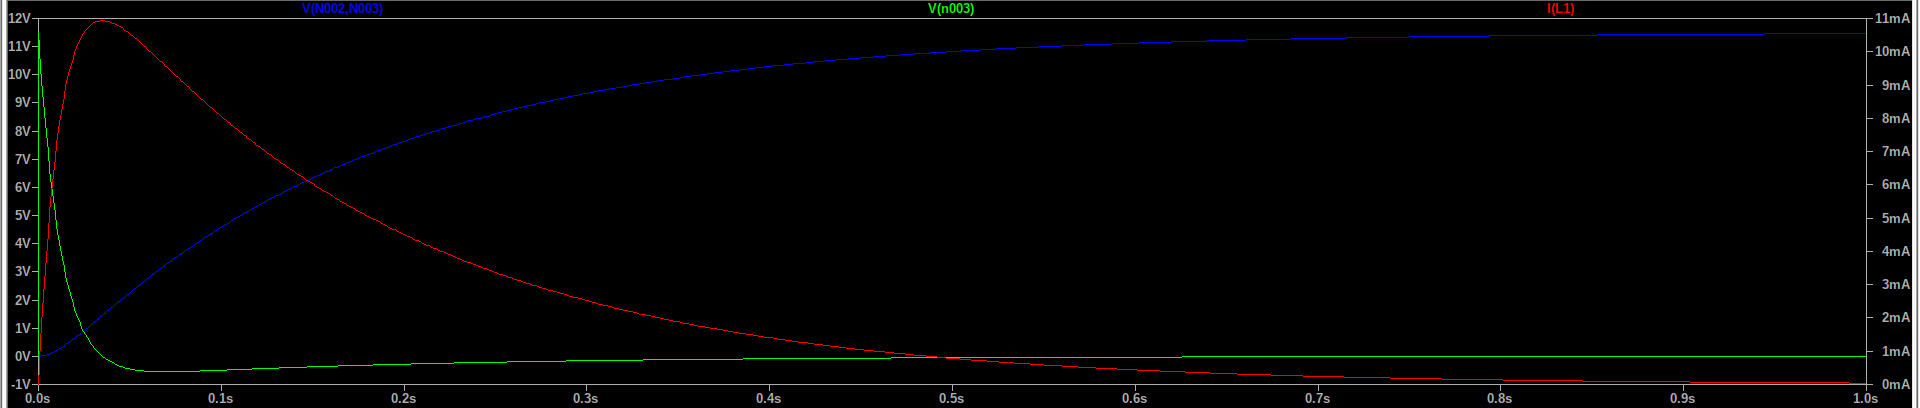
\includegraphics[width=19cm]{graphic2_1.png}
    \caption{График для апериодического процесса}
\end{figure}


\begin{figure}[H]
    \centering
    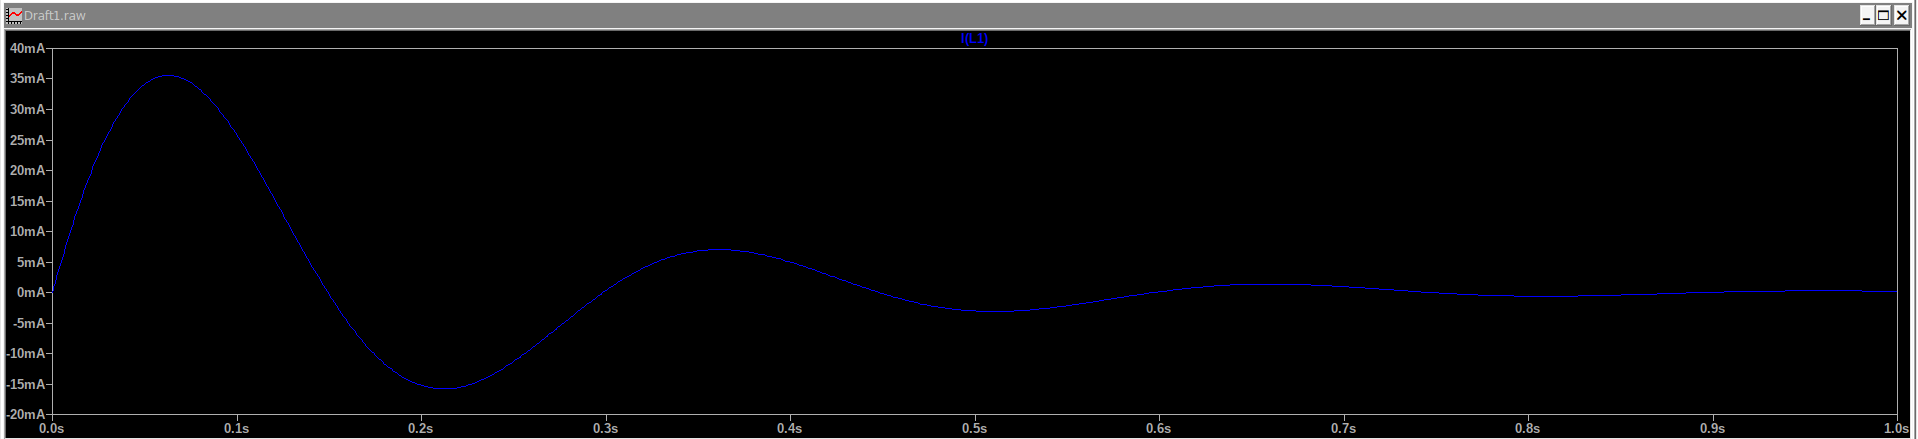
\includegraphics[width=19cm]{graphic2_2.png}
    \caption{График для колебательного}
\end{figure}


\newpage




\subsection*{Часть 3: Исследование переходного процесса в RL-цепи с источником переменного напряжения}

В данной части рассматривается подключение катушки индуктивности к источнику синусоидального напряжения $e(t) = E_m \sin(\omega t + \psi_e)$. Принимаем начальную фазу источника $\psi_e = 0$.

\begin{figure}[H]
    \centering
    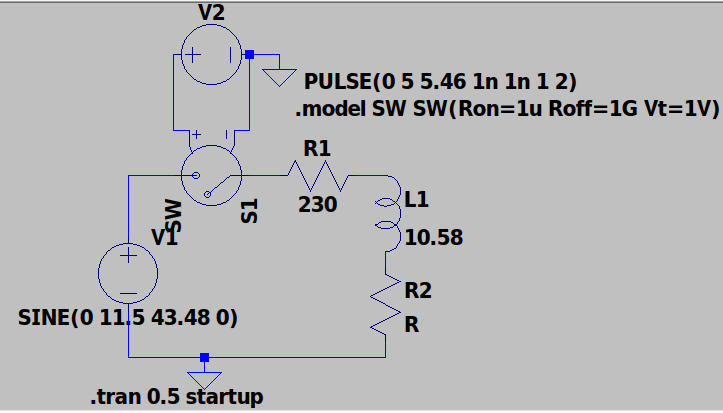
\includegraphics[width=12cm]{scheme3.png}
    \caption{Схема цепи}
\end{figure}

\subsubsection*{3.1 Расчет теоретических параметров (Таблица 4.7)}

\begin{enumerate}
    \item Постоянная времени цепи: 
    $$\tau = \frac{L}{R + R_k} = \frac{10.580}{230.000 + 0} = 0.046 \text{ с} = 46.000 \text{ мс.}$$
    \item Период напряжения для случая $T = \tau/2$: 
    $$T_1 = 0.023 \text{ с} \Rightarrow f_1 = \frac{1}{T_1} = 43.478 \text{ Гц.}$$
    \item Период напряжения для случая $T = 2\tau$: 
    $$T_2 = 0.092 \text{ с} \Rightarrow f_2 = \frac{1}{T_2} = 10.870 \text{ Гц.}$$
    \item Угол сдвига фаз $\phi$:
    \begin{itemize}
        \item При $f_1 = 43.478$ Гц: $\phi_1 = \text{arctg}\left(\frac{2\pi \cdot 43.478 \cdot 10.580}{230}\right) = \text{arctg}(12.566) = 85.451^\circ$ (1.491 рад).
        \item При $f_2 = 10.870$ Гц: $\phi_2 = \text{arctg}\left(\frac{2\pi \cdot 10.870 \cdot 10.580}{230}\right) = \text{arctg}(3.142) = 72.343^\circ$ (1.263 рад).
    \end{itemize}
\end{enumerate}

\begin{table}[H]
\centering
\caption{Параметры цепи и источника (Таблица 4.7)}
\begin{tabular}{|l|l|}
\hline
Переменная & Значение \\
\hline
$\tau$, [с] & 0.046 \\
\hline
$f$ при $T = \tau/2$, [Гц] & 43.478 \\
\hline
$f$ при $T = 2\tau$, [Гц] & 10.870 \\
\hline
$\phi$ при $T = \tau/2$, [град] & 85.451 \\
\hline
$\phi$ при $T = 2\tau$, [град] & 72.343 \\
\hline
\end{tabular}
\end{table}

\subsubsection*{3.2 Анализ максимальных значений тока (Таблица 4.8)}

На основании замеров определены максимальные амплитудные значения тока $i_{max}$ для различных углов включения $\alpha$.

\begin{table}[H]
\centering
\caption{Максимальные значения тока $i_{max}$, [мА] (Таблица 4.8)}
\begin{tabular}{|l|c|c|c|c|c|}
\hline
Режим & $\alpha = \phi$ & $\alpha = \phi - \pi/4$ & $\alpha = \phi + \pi/4$ & $\alpha = \phi + \pi/2$ & $\alpha = \pi$ \\
\hline
$T = \tau/2$ & 3.960 & 6.288 & 4.272 & 7.458 & 7.060 \\
\hline
$T = 2\tau$ & 15.163 & 15.119 & 15.088 & 20.312 & 11.463 \\ 
\hline
\end{tabular}
\end{table}


\begin{figure}[H]
    \centering
    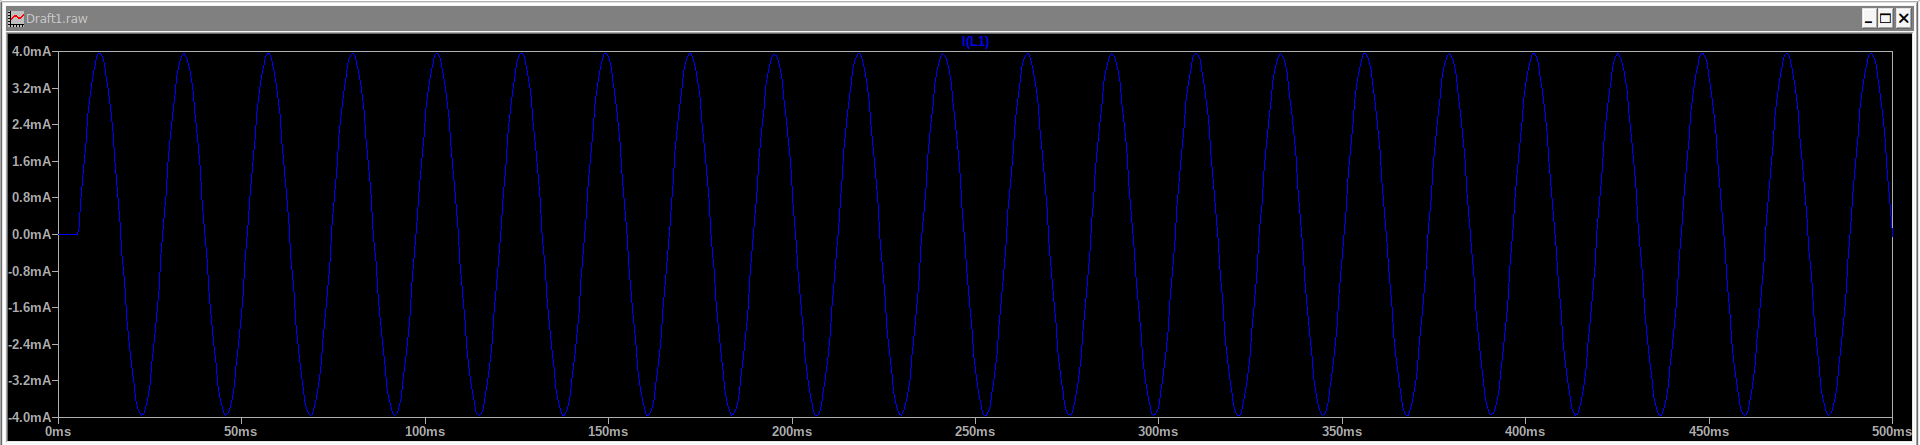
\includegraphics[width=19cm]{graphic3_1.png}
    \caption{График}
\end{figure}

\subsubsection*{Выводы по работе}
\begin{enumerate}
    \item В первой части работы подтверждены законы коммутации для $RC$ и $RL$ цепей. Экспериментальные значения постоянных времени $\tau$ практически совпали с расчетными (отклонение менее 0.5\%).
    \item Во второй части ($RLC$-цепь) продемонстрирована зависимость характера процесса от сопротивления $R$. При $R=920$ Ом ($R > 2\rho$) наблюдался апериодический процесс, а при $R=115$ Ом ($R < 2\rho$) — колебательный. 
    \item В третьей части установлено, что при включении цепи в момент $\alpha = \phi$ переходная составляющая минимальна, и ток сразу принимает установившееся значение. При отклонении угла включения от $\phi$ (наиболее выражено при $\alpha \approx \phi \pm \pi/2$) возникает "сверхток", амплитуда которого в переходном режиме может значительно превышать амплитуду установившегося тока. 
\end{enumerate}
\end{document}